
\documentclass[letterpaper,12pt]{article}

\usepackage{threeparttable}
\usepackage{geometry}
\geometry{letterpaper,tmargin=1in,bmargin=1in,lmargin=1.25in,rmargin=1.25in}
\usepackage[format=hang,font=normalsize,labelfont=bf]{caption}
\usepackage{amsmath}
\usepackage{multirow}
\usepackage{array}
\usepackage{delarray}
\usepackage{amssymb}
\usepackage{amsthm}
\usepackage{lscape}
\usepackage{natbib}
\usepackage{setspace}
\usepackage{float,color}
\usepackage[pdftex]{graphicx}
\usepackage{pdfsync}
\usepackage{verbatim}
\usepackage{placeins}
\usepackage{geometry}
\usepackage{pdflscape}
\synctex=1
\usepackage{hyperref}
\hypersetup{colorlinks,linkcolor=red,urlcolor=blue,citecolor=red}
\usepackage{bm}


\theoremstyle{definition}
\newtheorem{theorem}{Theorem}
\newtheorem{acknowledgement}[theorem]{Acknowledgement}
\newtheorem{algorithm}[theorem]{Algorithm}
\newtheorem{axiom}[theorem]{Axiom}
\newtheorem{case}[theorem]{Case}
\newtheorem{claim}[theorem]{Claim}
\newtheorem{conclusion}[theorem]{Conclusion}
\newtheorem{condition}[theorem]{Condition}
\newtheorem{conjecture}[theorem]{Conjecture}
\newtheorem{corollary}[theorem]{Corollary}
\newtheorem{criterion}[theorem]{Criterion}
\newtheorem{definition}{Definition} % Number definitions on their own
\newtheorem{derivation}{Derivation} % Number derivations on their own
\newtheorem{example}[theorem]{Example}
\newtheorem{exercise}[theorem]{Exercise}
\newtheorem{lemma}[theorem]{Lemma}
\newtheorem{notation}[theorem]{Notation}
\newtheorem{problem}[theorem]{Problem}
\newtheorem{proposition}{Proposition} % Number propositions on their own
\newtheorem{remark}[theorem]{Remark}
\newtheorem{solution}[theorem]{Solution}
\newtheorem{summary}[theorem]{Summary}
\bibliographystyle{aer}
\newcommand\ve{\varepsilon}
\renewcommand\theenumi{\roman{enumi}}
\newcommand\norm[1]{\left\lVert#1\right\rVert}

\begin{document}



Asset Pricing

\subsection*{Exercise 1}
I get a whole slew of answers, depending both on whether I use bounded or unbounded optimization and my guess. For the following guesses (left-hand column) using an unbounded optimization method, I got the following answers (right-hand column):

\[\text{Unbounded}\] 
\begin{align*}\\
    \text{Initial guess} [\beta,\gamma] &\implies \text{Parameter Values}[\beta,\gamma]\\
[.5,1] &\implies [ 0.99204351,  0.9981376 ]\\
[.5,5] &\implies [1.02223033,  4.99806877]\\
[.5,10] &\implies[ 1.06020221,  9.99799095]\\
[.1,1] &\implies[ 0.99205244,  0.99932601]\\
[.5,1] &\implies[ 0.99204351,  0.9981376 ]\\
[.9,1] &\implies[ 0.99205169,  0.99937255]\\
\end{align*}
\[\text{Bounded}\] 
\begin{align*}
    \text{Initial guess} [\beta,\gamma] &\implies \text{Parameter Values}[\beta,\gamma]\\
[.5,1] &\implies[ 1        ,  2.06584791]\\
[.5,5] &\implies[ 1        ,  2.06584775]\\
[.5,10] &\implies[ 1        ,  2.06584781]\\
[.1,1] &\implies[ 1        ,  2.06584823]\\
[.5,1] &\implies[ 1       ,  2.06584775]\\
[.9,1] &\implies[ 1        ,  2.06584783]\\
\end{align*}

There is no clear answer here, as is to be expected on a tough optimization problem. However, it seems that $\beta$ hovers pretty reliably around 1, meaning that there is not much of a discounting factor, if at all. This would be a reliable answer were people to value their future consumption as they do their current consumption. This is generally not the case, though, so these results seem odd to me. \\
\indent With the unbounded optimization, my answers for $\gamma$ seem to be bunk, as they change right along with the guess. As is seen in the figure below, though, we can see that the choice of $\gamma$ vary widely with a little change in $\beta$. We can be much more of the answers we've gotten for beta in the unbounded case. The closest thing we have to an answer for $\gamma$ is around $2.065$, as in the bounded case, we get this result regardless of our guess. \\
\indent Ultimately, I would make the following guesses:
\begin{align*}
\beta &\approx .99\\
\gamma&\approx 2.065\\
\end{align*} 
implying little discounting and relatively low risk-aversion.

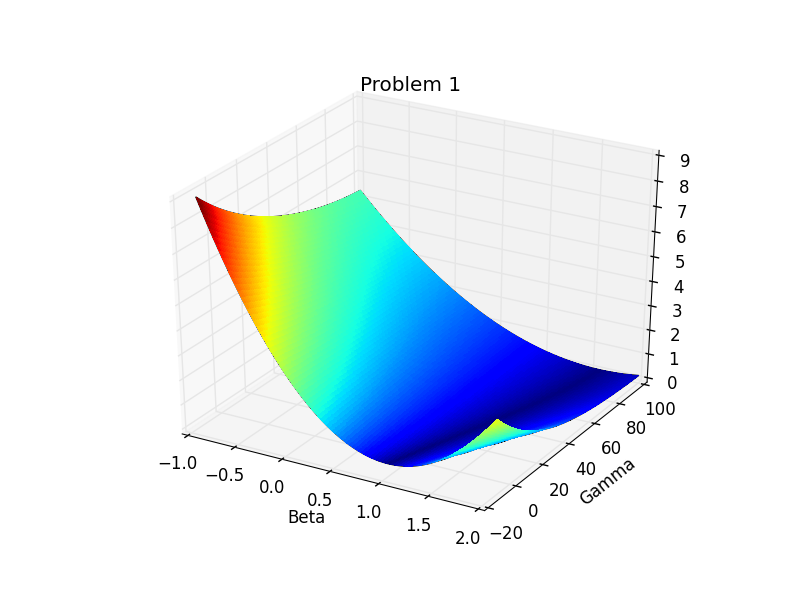
\includegraphics[scale = .75]{betagammafig.png}


\subsection*{Exercise 2}


\[\text{Parameter Values}\] 
\[[\beta,\alpha,\phi,\gamma] = [ 0.98291771,  0.01,  0.01,  0.00993389]\]

$\gamma \nrightarrow \infty$, so we know that the marginal investor does not have CARA preferences. It seems that $\gamma$ \textgreater $0$, thus the marginal investor could have incresing absolute risk tolerance. This also suggests the possibility of CRRA preferences, but this is a weak conclusion due to the fact that $\phi \neq 0$.\\
\indent There are obviously some issues here as well, that the parameter outcomes stay near the initial guesses. I anticipate that the reasons for this are similar to the Exercise 1, though, and due to this the results are dodgy. 

\subsection*{Exercise 3 (i)}


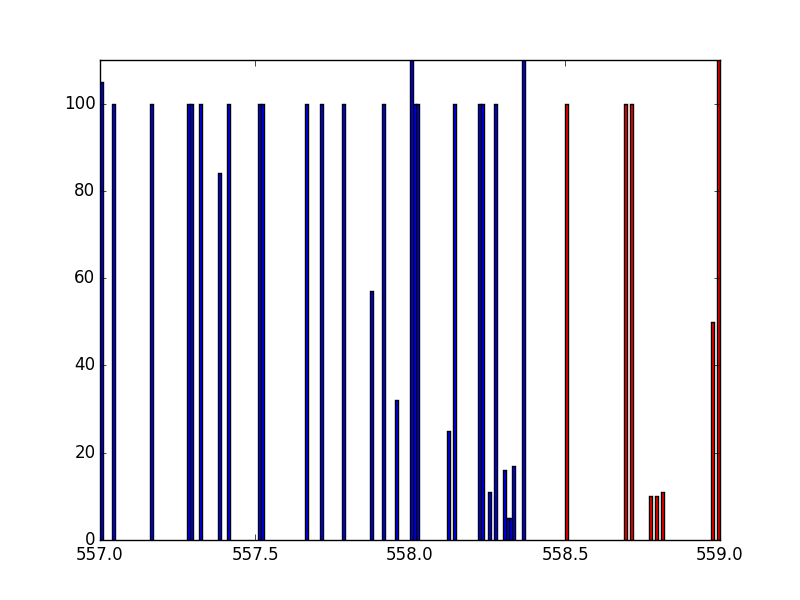
\includegraphics[scale = .75]{orderbook.png}

\subsection*{Exercise 3 (ii)}
Volume of shares transacted for Google on 6/23/14: 349388

\subsection*{Exercise 3 (iii)}
Average spread: 16.7142246903 cents

\subsection*{Exercise 3 (iv)}
Revenue of market makers: 30620.28

\subsection*{Exercise 3 (v)}
 
$.73\%$ is the likelihood of an informed trade


\end{document}
